\documentclass[]{book}
\usepackage{lmodern}
\usepackage{amssymb,amsmath}
\usepackage{ifxetex,ifluatex}
\usepackage{fixltx2e} % provides \textsubscript
\ifnum 0\ifxetex 1\fi\ifluatex 1\fi=0 % if pdftex
  \usepackage[T1]{fontenc}
  \usepackage[utf8]{inputenc}
\else % if luatex or xelatex
  \ifxetex
    \usepackage{mathspec}
  \else
    \usepackage{fontspec}
  \fi
  \defaultfontfeatures{Ligatures=TeX,Scale=MatchLowercase}
\fi
% use upquote if available, for straight quotes in verbatim environments
\IfFileExists{upquote.sty}{\usepackage{upquote}}{}
% use microtype if available
\IfFileExists{microtype.sty}{%
\usepackage{microtype}
\UseMicrotypeSet[protrusion]{basicmath} % disable protrusion for tt fonts
}{}
\usepackage[margin=1in]{geometry}
\usepackage{hyperref}
\hypersetup{unicode=true,
            pdftitle={Handout\_V2},
            pdfauthor={Pierre Bauche},
            pdfborder={0 0 0},
            breaklinks=true}
\urlstyle{same}  % don't use monospace font for urls
\usepackage{natbib}
\bibliographystyle{plainnat}
\usepackage{color}
\usepackage{fancyvrb}
\newcommand{\VerbBar}{|}
\newcommand{\VERB}{\Verb[commandchars=\\\{\}]}
\DefineVerbatimEnvironment{Highlighting}{Verbatim}{commandchars=\\\{\}}
% Add ',fontsize=\small' for more characters per line
\usepackage{framed}
\definecolor{shadecolor}{RGB}{248,248,248}
\newenvironment{Shaded}{\begin{snugshade}}{\end{snugshade}}
\newcommand{\KeywordTok}[1]{\textcolor[rgb]{0.13,0.29,0.53}{\textbf{#1}}}
\newcommand{\DataTypeTok}[1]{\textcolor[rgb]{0.13,0.29,0.53}{#1}}
\newcommand{\DecValTok}[1]{\textcolor[rgb]{0.00,0.00,0.81}{#1}}
\newcommand{\BaseNTok}[1]{\textcolor[rgb]{0.00,0.00,0.81}{#1}}
\newcommand{\FloatTok}[1]{\textcolor[rgb]{0.00,0.00,0.81}{#1}}
\newcommand{\ConstantTok}[1]{\textcolor[rgb]{0.00,0.00,0.00}{#1}}
\newcommand{\CharTok}[1]{\textcolor[rgb]{0.31,0.60,0.02}{#1}}
\newcommand{\SpecialCharTok}[1]{\textcolor[rgb]{0.00,0.00,0.00}{#1}}
\newcommand{\StringTok}[1]{\textcolor[rgb]{0.31,0.60,0.02}{#1}}
\newcommand{\VerbatimStringTok}[1]{\textcolor[rgb]{0.31,0.60,0.02}{#1}}
\newcommand{\SpecialStringTok}[1]{\textcolor[rgb]{0.31,0.60,0.02}{#1}}
\newcommand{\ImportTok}[1]{#1}
\newcommand{\CommentTok}[1]{\textcolor[rgb]{0.56,0.35,0.01}{\textit{#1}}}
\newcommand{\DocumentationTok}[1]{\textcolor[rgb]{0.56,0.35,0.01}{\textbf{\textit{#1}}}}
\newcommand{\AnnotationTok}[1]{\textcolor[rgb]{0.56,0.35,0.01}{\textbf{\textit{#1}}}}
\newcommand{\CommentVarTok}[1]{\textcolor[rgb]{0.56,0.35,0.01}{\textbf{\textit{#1}}}}
\newcommand{\OtherTok}[1]{\textcolor[rgb]{0.56,0.35,0.01}{#1}}
\newcommand{\FunctionTok}[1]{\textcolor[rgb]{0.00,0.00,0.00}{#1}}
\newcommand{\VariableTok}[1]{\textcolor[rgb]{0.00,0.00,0.00}{#1}}
\newcommand{\ControlFlowTok}[1]{\textcolor[rgb]{0.13,0.29,0.53}{\textbf{#1}}}
\newcommand{\OperatorTok}[1]{\textcolor[rgb]{0.81,0.36,0.00}{\textbf{#1}}}
\newcommand{\BuiltInTok}[1]{#1}
\newcommand{\ExtensionTok}[1]{#1}
\newcommand{\PreprocessorTok}[1]{\textcolor[rgb]{0.56,0.35,0.01}{\textit{#1}}}
\newcommand{\AttributeTok}[1]{\textcolor[rgb]{0.77,0.63,0.00}{#1}}
\newcommand{\RegionMarkerTok}[1]{#1}
\newcommand{\InformationTok}[1]{\textcolor[rgb]{0.56,0.35,0.01}{\textbf{\textit{#1}}}}
\newcommand{\WarningTok}[1]{\textcolor[rgb]{0.56,0.35,0.01}{\textbf{\textit{#1}}}}
\newcommand{\AlertTok}[1]{\textcolor[rgb]{0.94,0.16,0.16}{#1}}
\newcommand{\ErrorTok}[1]{\textcolor[rgb]{0.64,0.00,0.00}{\textbf{#1}}}
\newcommand{\NormalTok}[1]{#1}
\usepackage{longtable,booktabs}
\usepackage{graphicx,grffile}
\makeatletter
\def\maxwidth{\ifdim\Gin@nat@width>\linewidth\linewidth\else\Gin@nat@width\fi}
\def\maxheight{\ifdim\Gin@nat@height>\textheight\textheight\else\Gin@nat@height\fi}
\makeatother
% Scale images if necessary, so that they will not overflow the page
% margins by default, and it is still possible to overwrite the defaults
% using explicit options in \includegraphics[width, height, ...]{}
\setkeys{Gin}{width=\maxwidth,height=\maxheight,keepaspectratio}
\IfFileExists{parskip.sty}{%
\usepackage{parskip}
}{% else
\setlength{\parindent}{0pt}
\setlength{\parskip}{6pt plus 2pt minus 1pt}
}
\setlength{\emergencystretch}{3em}  % prevent overfull lines
\providecommand{\tightlist}{%
  \setlength{\itemsep}{0pt}\setlength{\parskip}{0pt}}
\setcounter{secnumdepth}{5}
% Redefines (sub)paragraphs to behave more like sections
\ifx\paragraph\undefined\else
\let\oldparagraph\paragraph
\renewcommand{\paragraph}[1]{\oldparagraph{#1}\mbox{}}
\fi
\ifx\subparagraph\undefined\else
\let\oldsubparagraph\subparagraph
\renewcommand{\subparagraph}[1]{\oldsubparagraph{#1}\mbox{}}
\fi

%%% Use protect on footnotes to avoid problems with footnotes in titles
\let\rmarkdownfootnote\footnote%
\def\footnote{\protect\rmarkdownfootnote}

%%% Change title format to be more compact
\usepackage{titling}

% Create subtitle command for use in maketitle
\newcommand{\subtitle}[1]{
  \posttitle{
    \begin{center}\large#1\end{center}
    }
}

\setlength{\droptitle}{-2em}
  \title{Handout\_V2}
  \pretitle{\vspace{\droptitle}\centering\huge}
  \posttitle{\par}
  \author{Pierre Bauche}
  \preauthor{\centering\large\emph}
  \postauthor{\par}
  \predate{\centering\large\emph}
  \postdate{\par}
  \date{2018-09-03}

\usepackage{booktabs}

\usepackage{amsthm}
\newtheorem{theorem}{Theorem}[chapter]
\newtheorem{lemma}{Lemma}[chapter]
\theoremstyle{definition}
\newtheorem{definition}{Definition}[chapter]
\newtheorem{corollary}{Corollary}[chapter]
\newtheorem{proposition}{Proposition}[chapter]
\theoremstyle{definition}
\newtheorem{example}{Example}[chapter]
\theoremstyle{definition}
\newtheorem{exercise}{Exercise}[chapter]
\theoremstyle{remark}
\newtheorem*{remark}{Remark}
\newtheorem*{solution}{Solution}
\begin{document}
\maketitle

{
\setcounter{tocdepth}{1}
\tableofcontents
}
\chapter{\texorpdfstring{\textbf{Information}}{Information}}\label{information}

\section{Usefull ressource}\label{usefull-ressource}

Feature engenering :
\url{http://www.feat.engineering/review-predictive-modeling-process.html}
Semi supervized learning :
\url{https://www.analyticsvidhya.com/blog/2017/09/pseudo-labelling-semi-supervised-learning-technique/}\\
- Machine Learning wth unlabbeled data : psuedo labeling

\begin{itemize}
\tightlist
\item
  Book

  \begin{itemize}
  \tightlist
  \item
    Artificial Intelligence: A Modern Approach" by Stuart Russell and
    Peter Norvig.
  \end{itemize}
\end{itemize}

\section{todo}\label{todo}

\begin{itemize}
\tightlist
\item
  create Blogdown
\item
  tydiverse package
\item
  Tensorflow for deep learning : open source software library developed
  at google for complex computation
\end{itemize}

\section{interesting stuff}\label{interesting-stuff}

\begin{itemize}
\item
  polynomial regression using kernel smoothing
\item
  Logistic regression using 5 fold stratified cross validation
\item
  blockchain data science
\item
  reinforcement learning
\item
  adversarial training -Deep Learning

  \begin{itemize}
  \tightlist
  \item
    microsoft service
  \item
    Tensorflow : read exemple
  \item
    RKWard : free and open source Graphical User Interface for the R
    software
  \end{itemize}
\item
  ML with H2O, lime, Keras
\item
  spark R
\item
  image recognizing with R
\item
  sentiment analysis = microsoft azure
\item
  data privacy
\item
  data quality control
\item
  Web developpement
\item
  Shiny : (microsoft azure serveur pour upload
\item
  Rmarckodw :
\item
  blogdown (Hugo)
\item
  Insurance
\item
  fraud
\item
  underwriting models : predict somebody's insurance risk
\item
  marketing predition
\item
  customer segmentation
\end{itemize}

\section{Hint}\label{hint}

\chapter{Feature engeneering}\label{feature-engeneering}

\section{Input feature}\label{input-feature}

A feature is a numeric representation of raw data. Feature engineering
is the process of formulating the most appropriate features given the
data, the model, and the task. If features are't good enought then model
canot be good.

Features selection is important. If they are to many fearture, model use
noise or irrelevant information or redundant. IF they are not enought
feature, model don't have the information .

\begin{itemize}
\tightlist
\item
  \textbf{Create new input :}

  \begin{itemize}
  \tightlist
  \item
    Combine feature

    \begin{itemize}
    \tightlist
    \item
      reduire dimention
    \item
      reduire colinéarité
    \item
      predictor qui ont du sens
    \item
      use the input interaction
    \end{itemize}
  \item
    kmeans clustering as feature : attetion pas inclure la target risque
    overfitting

    \begin{itemize}
    \tightlist
    \item
      a data point can also be represented by a dense vector of its
      inverse distance to each cluster center. This retains more
      information than simple binary cluster assignment
    \end{itemize}
  \item
    n-day average (in time series) : peut reduire la variabilite etle
    noise
  \item
    ratio
  \end{itemize}
\item
  \textbf{Tips}

  \begin{itemize}
  \tightlist
  \item
    Use knowledge to construct a better set of features (business)
  \item
    Visualizing the correlation and check de relation

    \begin{itemize}
    \tightlist
    \item
      between input and output when output is numeric
    \item
      between different input
    \end{itemize}
  \item
    Normalize the feature if metrics differt or unknow
  \end{itemize}
\end{itemize}

\subsection{Numeric Data}\label{numeric-data}

Predictors that are on a continuous scale are subject to somes issues
that can be mitigated through the choose of model. Models that are
smooth functions of input features or model hat use euclidian distance
(regression, clustering, \ldots{}) are sensitive to the scale. Models
based on space-partitioning trees (decision trees, gradient boosted
machines, random forests) are not sensitive to scale.

There are a variety of modifications that can be made to an individual
predictor that might improve its utility in a model.

\begin{itemize}
\tightlist
\item
  \textbf{scaling} : not change the shape of the distribution
  \(/frac{x-min(x)}{max(x)-min(x)}\)

  \begin{itemize}
  \tightlist
  \item
    Feature scaling is useful in situations where a set of input
    features differs wildly in scale.
  \end{itemize}
\item
  \textbf{standardization on N(0,1)} : \(/frac{x-mean(x)}{sqrt(var())}\)

  \begin{itemize}
  \tightlist
  \item
    essential when the distance or dot products between predictors are
    used (such as K-nearest neighbors or support vector machines)
  \item
    essential when the variables are required to be a a common scale in
    order to apply a penalty (e.g.~the lasso or ridge regression)
  \end{itemize}
\item
  \textbf{normalisation} : divide by the euclienne l² norme (=sums the
  squares of the values of the features across data points). SO the
  feature column has norm = 1
\item
  \textbf{Discretization} :

  \begin{itemize}
  \tightlist
  \item
    fixed width
  \item
    quantile binning
  \end{itemize}
\end{itemize}

\begin{quote}
Variables scaled and standardized are comparable Some models need
gaussian input : scale + transform
\end{quote}

\begin{itemize}
\tightlist
\item
  \textbf{Power transforms} : variance-stabilizing transformations**
  Power transforms change the distribution of the variable to more
  symetric distribution

  \begin{itemize}
  \tightlist
  \item
    log
  \item
    sqrt
  \item
    inverse
  \item
    boxcox : generalisation : Only work for positive variable
  \item
    johnson transform
  \item
    logit transformations : This transformation changes the scale from
    zero and one to values between negative and positive infinity
  \end{itemize}
\end{itemize}

\subsection{count data}\label{count-data}

Raw counts that span several orders of magnitude are problematic for
many models.In a linear model, the same linear coefficient would have to
work for all possible values of the count. Large counts could also wreak
havoc in unsupervised learning methods such as k-means clustering, which
uses Euclidean distance as a similarity function to measure the
similarity between data points. A large count in one element of the data
vector would outweigh the similarity in all other elements, which could
throw off the entire similarity measurement.

\begin{itemize}
\tightlist
\item
  \textbf{count transform}

  \begin{itemize}
  \tightlist
  \item
    binarise 0/1 if value
  \item
    quantizing the count or group the counts

    \begin{itemize}
    \tightlist
    \item
      fixed-width binning, each bin contains a specific numeric range
      (ex age)
    \item
      If count have multiple magnitudes, group by powers of 10 ( 0--9,
      10--99, 100--999, 1000--9999, etc)
    \end{itemize}
  \item
    Quantile binning : adaptively positioning the bins based on the
    distribution of the data
  \item
    log transform
  \end{itemize}
\end{itemize}

\subsection{categorical data}\label{categorical-data}

Use Dummy or keep factors with somes levels is same for most modeling.
It suggest using the predictors without converting to dummy variables
and, if the model appears promising, to also try refitting using dummy
variables.

\begin{itemize}
\tightlist
\item
  \textbf{unordered categorical data}

  \begin{itemize}
  \tightlist
  \item
    dummy coding : in Feature engineering, il recommande de flag chaque
    variable categorielle en varible binaire
  \item
    effect coding : -1 0 1 : -1 si different de categorie de reference.
    Effect coding is very similar to dummy coding, but results in linear
    regression models that are even simpler to interpret.
  \end{itemize}
\item
  \textbf{Dealing with Large Categorical Variables}

  \begin{itemize}
  \tightlist
  \item
    do nothing
  \item
    dummy : create many variable with zero value for rare categories and
    add zero-variance predictor( computentional intencive )
  \item
    delete rare value
  \item
    recode and regroup categorical data
  \item
    Compress the features. There are two choices:

    \begin{itemize}
    \tightlist
    \item
      Feature hashing, popular with linear models. A hash function is a
      deterministic function that maps a potentially unbounded integer
      to a finite integer range {[}1, m{]}. Feature hashing compresses
      the original feature vector into an m-dimensional vector. It
      Converte large cat var into small hash feature (but hashing
      feature are uninterpretable)
    \item
      Bin counting, popular with linear models as well as trees. Rather
      than using the value of the categorical variable as the feature,
      use the conditional probability of the target under that value. In
      other words, instead of encoding the identity of the categorical
      value, we compute the association statistics between that value
      and the target that we wish to predict
    \end{itemize}
  \end{itemize}
\item
  \textbf{Ordered data}

  \begin{itemize}
  \tightlist
  \item
    how measure de force to pass between each categorie ?

    \begin{itemize}
    \tightlist
    \item
      linear
    \item
      quadratic
    \end{itemize}
  \end{itemize}
\end{itemize}

\subsection{Date Time : Lubridate
package}\label{date-time-lubridate-package}

\begin{itemize}
\tightlist
\item
  Use as.POSIXct() and UTC (universal coordinated time)in time zone.
\item
  create new variables : weekend (0/1), bankholiday (0/1), \ldots{}
\end{itemize}

\section{Missing Value}\label{missing-value}

\begin{itemize}
\tightlist
\item
  Do nothing
\item
  remove
\item
  impute

  \begin{itemize}
  \tightlist
  \item
    by mean : doesn't impact analysis
  \item
    by singular value decomposition : approximate true value
  \item
    by regression :approximate true value
  \item
    Check lien 5 methode impute missing value
  \end{itemize}
\end{itemize}

\section{Outlier Detection}\label{outlier-detection}

\section{Sampling and resampling}\label{sampling-and-resampling}

Modern statistical methods assume that the underlying data comes from a
random distribution. The performance measurements of models derived from
data are also subject to random noise. the sample can be generalized for
the population with statistical confidence. Is an approximatation.

\begin{quote}
Weak law of large numbers : \(\bar{X_n} => \mu\)\\
Central limit theorem : distribution standardis? tend vers une normale
asymptotiquement
\end{quote}

\begin{itemize}
\tightlist
\item
  \textbf{model sampling} : population data is already collected and you
  want to reduce time and the computational cost of analysis, along with
  improve the inference of your models
\item
  \textbf{survey sampling} : create a sample design and then survey the
  population only to collect sample to save data collection costs.
\end{itemize}

Type of sampling methods :

\begin{itemize}
\tightlist
\item
  Boostrap sampling : sampling with replacement
\item
  Jackknife = leave one out sampling + calculate average of the
  estimation
\item
  Vfold crossvalidation : Resampling methods that can generate V
  different versions of the training set (same size) that can be used to
  evaluate model on test set. Each of the V assessment sets contains 1/V
  of the training set and each of these exclude different data points.
  Suppose V = 10, then there are 10 different versions of 90\% of the
  data and also 10 versions of the remaining 10\% for each corresponding
  resample. in the end, there are V estimates of performance for the
  model and each was calculated on a different assessment set. The
  cross-validation estimate of performance is computed by averaging the
  V individual metrics.
\item
  Monte Carlo : Produces splits that are likely to contain overlap. For
  each resample, a random sample is taken with π proportion of the
  training set going into the analysis set and the remaining samples
  allocated to the assessment set
\item
  bootstrap : A bootstrap resample of the data is defined to be a simple
  random sample that is the same size as the training set where the data
  are sampled with replacement
\end{itemize}

\section{variables selections}\label{variables-selections}

How do we cleanly separate the signal from the noise?

\textbf{First Filter}

\begin{itemize}
\tightlist
\item
  Na filter : column with to many NA
\item
  Variance filter : Column with not enought variance to explain dataset
\item
  corrélation filter : e will remove predictors that are highly
  correlated (r2 \textgreater{} 0.9) with other predictors. see corrplot
\item
  Variance treshold : Variable with high variability also have higher
  information in them. We remove all variables havant variance less than
  a treshold.
\end{itemize}

\subsection{Filter methods :}\label{filter-methods}

Select variables sans modélisation. Methode univariée. Order feature by
importance. Methode robust contre overfitting mais peut selectionner
variables redondantes. It is best to do prefiltering conservatively, so
as not to inadvertently eliminate useful features before they even make
it to the model training step

\begin{itemize}
\tightlist
\item
  Chi square test
\item
  Correlation coefficients
\item
  information gain metrics
\item
  fisher score
\item
  variance treshold
\end{itemize}

\subsection{Wrapper Methods:}\label{wrapper-methods}

Test differentes combinaisons de feature selon crit?re de performance.
Predictive model is used to evaluate the set of feature by accurancy
metric. Méthode efficace pour la mod?lisation. Peut causé de
l'overfitting.

\begin{itemize}
\tightlist
\item
  forward/backward selection
\item
  recursive feature elimation algorithm
\item
  \ldots{}
\end{itemize}

\subsection{Embedded Methods :}\label{embedded-methods}

Next step to wrapper methods. Introduce a penalty factor to the
evaluation criteria of the model to bias the model toward lower
complexity. Balance between complexity and accurancy. Less
computationally expensive than Wrapper. Less prone to overfitting. These
methods perform feature selection as part of the model training process

\begin{itemize}
\tightlist
\item
  Lasso
\item
  Ridge regression
\item
  \ldots{}
\item
  Decision tree
\item
  Gradiant descent methods
\end{itemize}

\subsection{Dimension reduction :}\label{dimension-reduction}

See unsuppervized section

\begin{itemize}
\tightlist
\item
  PCA see unsupervised analysis : Due to the orthogonality constraint in
  the objective function, PCA transformation produces a nice side
  effect: the transformed features are no longer correlated.
\item
  svd
\item
  k-means as a featurization procedure, a data point can be represented
  by its cluster membership
\end{itemize}

\section{Example}\label{example}

\subsection{Credit risk modeling}\label{credit-risk-modeling}

\begin{itemize}
\tightlist
\item
  \textbf{Feature ranking}

  \begin{itemize}
  \tightlist
  \item
    Fit logistic model
  \item
    Calculate Gini coefficient
  \item
    rearrange variables ? combine, weighted sums, etc
  \item
    Need to understand variable individually ? use Filtering method
  \item
    data dirty ? detect outlier
  \item
    Data selection? use first ranking, forward selection and last
    Embedded method. Compare with crit?rion (misclassi, MSE, AIC, etc)
  \item
    improve performance? bootstrap : subsample your data et redo
    analysis
  \end{itemize}
\end{itemize}

\begin{Shaded}
\begin{Highlighting}[]
\NormalTok{### Data Prep }\AlertTok{###}
\NormalTok{#################}
\KeywordTok{library}\NormalTok{(MLmetrics)}

\NormalTok{data =}\StringTok{ }\KeywordTok{get}\NormalTok{(}\KeywordTok{load}\NormalTok{(}\StringTok{"C:/Users/007/Desktop/Data science with R/R/Dataset/LoanDefaultPred.RData"}\NormalTok{))}

\CommentTok{#Create the default variable}
\NormalTok{data[,}\StringTok{"default"}\NormalTok{]=}\KeywordTok{ifelse}\NormalTok{(data}\OperatorTok{$}\NormalTok{loss }\OperatorTok{==}\DecValTok{0}\NormalTok{, }\DecValTok{0}\NormalTok{,}\DecValTok{1}\NormalTok{)}
\KeywordTok{print}\NormalTok{(}\KeywordTok{table}\NormalTok{(data}\OperatorTok{$}\NormalTok{default)}\OperatorTok{*}\DecValTok{100}\OperatorTok{/}\KeywordTok{nrow}\NormalTok{(data))}
\end{Highlighting}
\end{Shaded}

\begin{verbatim}
## 
##      0      1 
## 90.635  9.365
\end{verbatim}

\begin{Shaded}
\begin{Highlighting}[]
\CommentTok{# Without prior kwowledge : if more than 30 variable is continuous}
\NormalTok{continuous <-}\KeywordTok{character}\NormalTok{()}
\NormalTok{categorical <-}\KeywordTok{character}\NormalTok{()}
\NormalTok{i =}\StringTok{ }\KeywordTok{names}\NormalTok{(data)[}\DecValTok{1}\NormalTok{]}
\NormalTok{p<-}\DecValTok{1}
\NormalTok{q<-}\DecValTok{1}

\ControlFlowTok{for}\NormalTok{ (i }\ControlFlowTok{in} \KeywordTok{names}\NormalTok{(data))\{}
\NormalTok{unique_levels =}\KeywordTok{length}\NormalTok{(}\KeywordTok{unique}\NormalTok{(data[,i]))}

  \ControlFlowTok{if}\NormalTok{(i }\OperatorTok\StringTok{ }\KeywordTok{c}\NormalTok{(}\StringTok{"id"}\NormalTok{,}\StringTok{"loss"}\NormalTok{,}\StringTok{"default"}\NormalTok{))\{}
\ControlFlowTok{next}\NormalTok{;}
\NormalTok{      \}}\ControlFlowTok{else} \ControlFlowTok{if}\NormalTok{ (unique_levels }\OperatorTok{<=}\DecValTok{30} \OperatorTok{|}\KeywordTok{is.character}\NormalTok{(data[,i]))\{}
\NormalTok{            categorical[p] <-i}
\NormalTok{            p=p}\OperatorTok{+}\DecValTok{1}
\NormalTok{            data[[i]] <-}\KeywordTok{factor}\NormalTok{(data[[i]])}
\NormalTok{  \}}\ControlFlowTok{else}\NormalTok{\{}
\NormalTok{            continuous[q] <-i}
\NormalTok{            q=q}\OperatorTok{+}\DecValTok{1}
\NormalTok{  \}\}}

\KeywordTok{cat}\NormalTok{(}\StringTok{"}\CharTok{\textbackslash{}n}\StringTok{Total number of continuous variables in feature set "}\NormalTok{,}\KeywordTok{length}\NormalTok{(continuous) }\OperatorTok{-}\DecValTok{1}\NormalTok{)}
\end{Highlighting}
\end{Shaded}

\begin{verbatim}
## 
## Total number of continuous variables in feature set  714
\end{verbatim}

\begin{Shaded}
\begin{Highlighting}[]
\KeywordTok{cat}\NormalTok{(}\StringTok{"}\CharTok{\textbackslash{}n}\StringTok{Total number of categorical variable in feature set "}\NormalTok{,}\KeywordTok{length}\NormalTok{(categorical) }\OperatorTok{-}\DecValTok{2}\NormalTok{)}
\end{Highlighting}
\end{Shaded}

\begin{verbatim}
## 
## Total number of categorical variable in feature set  52
\end{verbatim}

\begin{Shaded}
\begin{Highlighting}[]
\CommentTok{# Gini coef}
\NormalTok{performance_metric_gini <-}\KeywordTok{data.frame}\NormalTok{(}\DataTypeTok{feature =}\KeywordTok{character}\NormalTok{(), }\DataTypeTok{Gini_value =}\KeywordTok{numeric}\NormalTok{())}

\CommentTok{# for (feature in names(data))\{}
\CommentTok{#     if(feature %in%c("id","loss","default")) \{}
\CommentTok{#         next}
\CommentTok{#       \} else \{}
\CommentTok{# tryCatch(}
\CommentTok{#   \{glm_model <-glm(default ~get(feature),data=data,family=binomial(link="logit"));}
\CommentTok{#   predicted_values <-predict.glm(glm_model,newdata=data,type="response");}
\CommentTok{#   Gini_value <-Gini(predicted_values,data$default);}
\CommentTok{#   performance_metric_gini <-rbind(performance_metric_gini,cbind(feature,Gini_value));\},error=function(e)\{\})}
\CommentTok{# \}}
\CommentTok{# \}}
\CommentTok{# }
\CommentTok{# saveRDS(performance_metric_gini, "performance_metric_gini.rds")}
\NormalTok{performance_metric_gini <-}\StringTok{ }\KeywordTok{readRDS}\NormalTok{(}\StringTok{"./save/performance_metric_gini.rds"}\NormalTok{)}

\NormalTok{performance_metric_gini}\OperatorTok{$}\NormalTok{Gini_value <-}\KeywordTok{as.numeric}\NormalTok{(}\KeywordTok{as.character}\NormalTok{(performance_metric_gini}\OperatorTok{$}\NormalTok{Gini_value))}

\NormalTok{Ranked_Features <-performance_metric_gini[}\KeywordTok{order}\NormalTok{(}\OperatorTok{-}\NormalTok{performance_metric_gini}\OperatorTok{$}\NormalTok{Gini_value),]}
\KeywordTok{head}\NormalTok{(Ranked_Features)}
\end{Highlighting}
\end{Shaded}

\begin{verbatim}
##     feature Gini_value
## 389    f404  0.2579189
## 710    f766  0.2578312
## 585    f630  0.2415352
## 584    f629  0.2354368
## 321    f333  0.2352707
## 56      f64  0.2348747
\end{verbatim}

\begin{Shaded}
\begin{Highlighting}[]
\CommentTok{# Note  : When you are running loops over large datasets, it is possible that the loop might stop due to some errors. to escape that, consider using the trycatch() function in r}

\NormalTok{###################################################}
\NormalTok{### Try logistic regression with top 5 features }\AlertTok{###}
\NormalTok{###################################################}

\NormalTok{glm_model <-}\KeywordTok{glm}\NormalTok{(default }\OperatorTok{~}\NormalTok{f766 }\OperatorTok{+}\NormalTok{f404 }\OperatorTok{+}\NormalTok{f629 }\OperatorTok{+}\NormalTok{f630 }\OperatorTok{+}\NormalTok{f281 }\OperatorTok{+}\NormalTok{f322,}\DataTypeTok{data=}\NormalTok{data,}\DataTypeTok{family=}\KeywordTok{binomial}\NormalTok{(}\DataTypeTok{link=}\StringTok{"logit"}\NormalTok{))}
\NormalTok{predicted_values <-}\KeywordTok{predict.glm}\NormalTok{(glm_model,}\DataTypeTok{newdata=}\NormalTok{data,}\DataTypeTok{type=}\StringTok{"response"}\NormalTok{)}
\NormalTok{Gini_value <-}\KeywordTok{Gini}\NormalTok{(predicted_values,data}\OperatorTok{$}\NormalTok{default)}
\KeywordTok{summary}\NormalTok{(glm_model)}
\end{Highlighting}
\end{Shaded}

\begin{verbatim}
## 
## Call:
## glm(formula = default ~ f766 + f404 + f629 + f630 + f281 + f322, 
##     family = binomial(link = "logit"), data = data)
## 
## Deviance Residuals: 
##     Min       1Q   Median       3Q      Max  
## -0.6928  -0.4946  -0.4102  -0.3329   3.0013  
## 
## Coefficients:
##              Estimate Std. Error z value Pr(>|z|)  
## (Intercept) -1.502550   4.939282  -0.304   0.7610  
## f766        -0.010228   4.916519  -0.002   0.9983  
## f404        -1.395602   4.908606  -0.284   0.7762  
## f629        -0.306456   0.172632  -1.775   0.0759 .
## f630        -0.165047   0.128300  -1.286   0.1983  
## f281         0.007759   0.019386   0.400   0.6890  
## f322         0.264196   0.128472   2.056   0.0397 *
## ---
## Signif. codes:  0 '***' 0.001 '**' 0.01 '*' 0.05 '.' 0.1 ' ' 1
## 
## (Dispersion parameter for binomial family taken to be 1)
## 
##     Null deviance: 12415  on 19938  degrees of freedom
## Residual deviance: 12040  on 19932  degrees of freedom
##   (61 observations deleted due to missingness)
## AIC: 12054
## 
## Number of Fisher Scoring iterations: 5
\end{verbatim}

\begin{Shaded}
\begin{Highlighting}[]
\NormalTok{Gini_value}
\end{Highlighting}
\end{Shaded}

\begin{verbatim}
## [1] 0.2697868
\end{verbatim}

\begin{Shaded}
\begin{Highlighting}[]
\CommentTok{# Every features aren't always significant. Indication that features themselves are highly correlated. Gini coef has not improved. So investigate multicorrelation.}
\CommentTok{# Variable ranking method is univariate and lead to the selection of a redundant variables. }

\NormalTok{top_6_feature <-}\KeywordTok{data.frame}\NormalTok{(data}\OperatorTok{$}\NormalTok{f766,data}\OperatorTok{$}\NormalTok{f404,data}\OperatorTok{$}\NormalTok{f629,data}\OperatorTok{$}\NormalTok{f630,data}\OperatorTok{$}\NormalTok{f281,data}\OperatorTok{$}\NormalTok{f322)}
\KeywordTok{cor}\NormalTok{(top_6_feature, }\DataTypeTok{use=}\StringTok{"complete"}\NormalTok{)}
\end{Highlighting}
\end{Shaded}

\begin{verbatim}
##            data.f766  data.f404  data.f629  data.f630  data.f281
## data.f766  1.0000000  0.9996754  0.6777553  0.6378040  0.8205665
## data.f404  0.9996754  1.0000000  0.6774434  0.6374457  0.8204153
## data.f629  0.6777553  0.6774434  1.0000000  0.9155376  0.6628148
## data.f630  0.6378040  0.6374457  0.9155376  1.0000000  0.6202698
## data.f281  0.8205665  0.8204153  0.6628148  0.6202698  1.0000000
## data.f322 -0.7706228 -0.7707861 -0.5450001 -0.5048133 -0.7371242
##            data.f322
## data.f766 -0.7706228
## data.f404 -0.7707861
## data.f629 -0.5450001
## data.f630 -0.5048133
## data.f281 -0.7371242
## data.f322  1.0000000
\end{verbatim}

\subsection{variance treshold
approach}\label{variance-treshold-approach}

\begin{Shaded}
\begin{Highlighting}[]
\CommentTok{# Attention, les variables ne sont pas standardisées, on ne peut pas les comparer directement. On utilise le coeficient de variation :$c= \textbackslash{}fraq\{\textbackslash{}sigma\}\{\textbackslash{}mu\}$}

\CommentTok{# Calculate CV}
\NormalTok{coefficient_of_variance <-}\KeywordTok{data.frame}\NormalTok{(}\DataTypeTok{feature =}\KeywordTok{character}\NormalTok{(), }\DataTypeTok{cov =}\KeywordTok{numeric}\NormalTok{())}

\ControlFlowTok{for}\NormalTok{ (feature }\ControlFlowTok{in} \KeywordTok{names}\NormalTok{(data))\{}
  \ControlFlowTok{if}\NormalTok{(feature }\OperatorTok\KeywordTok{c}\NormalTok{(}\StringTok{"id"}\NormalTok{,}\StringTok{"loss"}\NormalTok{,}\StringTok{"default"}\NormalTok{))\{}\ControlFlowTok{next}
\NormalTok{  \}}\ControlFlowTok{else} \ControlFlowTok{if}\NormalTok{(feature }\OperatorTok\StringTok{ }\NormalTok{continuous)\{}
    \KeywordTok{tryCatch}\NormalTok{(\{}
\NormalTok{      cov <-}\KeywordTok{abs}\NormalTok{(}\KeywordTok{sd}\NormalTok{(data[[feature]], }\DataTypeTok{na.rm =}\OtherTok{TRUE}\NormalTok{)}\OperatorTok{/}\KeywordTok{mean}\NormalTok{(data[[feature]],}\DataTypeTok{na.rm =}\OtherTok{TRUE}\NormalTok{));}
      \ControlFlowTok{if}\NormalTok{(cov }\OperatorTok{!=}\OtherTok{Inf}\NormalTok{)\{}
\NormalTok{coefficient_of_variance <-}\KeywordTok{rbind}\NormalTok{(coefficient_of_variance,}\KeywordTok{cbind}\NormalTok{(feature, cov));}
\NormalTok{      \} }\ControlFlowTok{else}\NormalTok{ \{}\ControlFlowTok{next}\NormalTok{\}}
\NormalTok{              \},}\DataTypeTok{error=}\ControlFlowTok{function}\NormalTok{(e)\{\})}
\NormalTok{  \}}\ControlFlowTok{else}\NormalTok{\{}\ControlFlowTok{next}\NormalTok{\}}
\NormalTok{\}}

\NormalTok{coefficient_of_variance}\OperatorTok{$}\NormalTok{cov <-}\KeywordTok{as.numeric}\NormalTok{(}\KeywordTok{as.character}\NormalTok{(coefficient_of_variance}\OperatorTok{$}\NormalTok{cov))}
\NormalTok{Ranked_Features_cov <-coefficient_of_variance[}\KeywordTok{order}\NormalTok{(}\OperatorTok{-}\NormalTok{coefficient_of_variance}\OperatorTok{$}\NormalTok{cov),]}

\KeywordTok{head}\NormalTok{(Ranked_Features_cov)}
\end{Highlighting}
\end{Shaded}

\begin{verbatim}
##     feature       cov
## 294    f338 128.05980
## 377    f422 111.93083
## 664    f724  69.64913
## 349    f393  55.39446
## 712    f775  47.64456
## 350    f394  46.68719
\end{verbatim}

\begin{Shaded}
\begin{Highlighting}[]
\NormalTok{## Logistic model}

\NormalTok{glm_model <-}\KeywordTok{glm}\NormalTok{(default }\OperatorTok{~}\NormalTok{f338 }\OperatorTok{+}\NormalTok{f422 }\OperatorTok{+}\NormalTok{f724 }\OperatorTok{+}\NormalTok{f636 }\OperatorTok{+}\NormalTok{f775 }\OperatorTok{+}\NormalTok{f723,}\DataTypeTok{data=}\NormalTok{data, }\DataTypeTok{family=}\KeywordTok{binomial}\NormalTok{(}\DataTypeTok{link=}\StringTok{"logit"}\NormalTok{));}
\NormalTok{predicted_values <-}\KeywordTok{predict.glm}\NormalTok{(glm_model,}\DataTypeTok{newdata=}\NormalTok{data,}\DataTypeTok{type=}\StringTok{"response"}\NormalTok{)}
\NormalTok{Gini_value <-}\KeywordTok{Gini}\NormalTok{(predicted_values,data}\OperatorTok{$}\NormalTok{default)}

\KeywordTok{cat}\NormalTok{(}\StringTok{"The Gini Coefficient for the fitted model is "}\NormalTok{,Gini_value);}
\end{Highlighting}
\end{Shaded}

\begin{verbatim}
## The Gini Coefficient for the fitted model is  0.1465253
\end{verbatim}

Contrairement au Ranking avec Gini, les variables ne sont pas dominés
par leur structure de correlation. Mais les variables ne sont pas toutes
significatives individuellement et le coef GINI pas particuliérement
amélioré. Avec variance treshlod on espére selectionné des variables
indépendantes

\section{Method Summary}\label{method-summary}

\begin{longtable}[]{@{}lll@{}}
\toprule
\begin{minipage}[b]{0.05\columnwidth}\raggedright\strut
\strut
\end{minipage} & \begin{minipage}[b]{0.22\columnwidth}\raggedright\strut
Variable quanti\strut
\end{minipage} & \begin{minipage}[b]{0.20\columnwidth}\raggedright\strut
Variable quali\strut
\end{minipage}\tabularnewline
\midrule
\endhead
\begin{minipage}[t]{0.05\columnwidth}\raggedright\strut
Graph\strut
\end{minipage} & \begin{minipage}[t]{0.22\columnwidth}\raggedright\strut
Time series, barplot, boxplot, histographe, QQplot, scaterplot\strut
\end{minipage} & \begin{minipage}[t]{0.20\columnwidth}\raggedright\strut
barplot, boxplot\strut
\end{minipage}\tabularnewline
\begin{minipage}[t]{0.05\columnwidth}\raggedright\strut
Test\strut
\end{minipage} & \begin{minipage}[t]{0.22\columnwidth}\raggedright\strut
t-test sur la moyenne, chi2 sur la variance, test normalité,
corrélation, test F variance, test de levene\strut
\end{minipage} & \begin{minipage}[t]{0.20\columnwidth}\raggedright\strut
test proportion, test ajustement, test indépendance\strut
\end{minipage}\tabularnewline
\begin{minipage}[t]{0.05\columnwidth}\raggedright\strut
Modélisation\strut
\end{minipage} & \begin{minipage}[t]{0.22\columnwidth}\raggedright\strut
Régression linéaire\strut
\end{minipage} & \begin{minipage}[t]{0.20\columnwidth}\raggedright\strut
régression logistique, analyse discriminante, abre décision\strut
\end{minipage}\tabularnewline
\bottomrule
\end{longtable}

\begin{itemize}
\tightlist
\item
  \textbf{Parametric} : assume thaht sample data is drawn from a known
  probabilité distribution based on fixed set of parameters. For
  instance, linear regression assumes normal distribution, whereas
  logistic assumes binomial distribution, etc. This assumption allows
  the methods to be applied to small datasets as well.

  \begin{itemize}
  \tightlist
  \item
    involve a two-step model-based approach : Chose model (ex : linear)
    and estimate (ex: ols)
  \item
    reduce the probleme of model estimation to a probleme of parameter
    estimation
  \item
    but if the chosen model is too far from the true f, then the
    estimate will be poor
  \end{itemize}
\item
  \textbf{Non parametric} : not assume any probabilty distribution or
  prior. Contruct empirical distributions from data. (= Kernel
  regression, NPMR)
\end{itemize}

Models can also be evaluated in terms of variance and bias.

\begin{itemize}
\tightlist
\item
  A model has high variance if small changes to the underlying data used
  to estimate the parameters cause a sizable change in those parameters
  (or in the structure of the model)
\item
  Model bias reflects the ability of a model to conform to the
  underlying theoretical structure of the data. A low bias model is one
  that can be highly flexible and has the capacity to fit a variety of
  different shapes and patterns. A high bias model would be unable to
  estimate values close to their true theoretical counterparts. Linear
  methods often have high bias since, without modification, cannot
  describe nonlinear patterns in the predictor variables. Tree-based
  models, support vector machines, neural networks, and others can be
  very adaptable to the data and have low bias.
\end{itemize}

\section{tips}\label{tips}

\begin{itemize}
\tightlist
\item
  Tidyverse package
\item
  Given below are some of the rare feature engineering tricks
  implemented in the winning solutions of several data science
  competitions. - Transform data to Image - Meta-leaks - Representation
  learning features Mean encodings - Transforming target variable
\end{itemize}

\chapter{Data visualization}\label{data-visualization}

\section{Descriptive}\label{descriptive}

\begin{Shaded}
\begin{Highlighting}[]
\CommentTok{#change theme => + theme()}

\NormalTok{iris }\OperatorTok\StringTok{ }\KeywordTok{qplot}\NormalTok{(Petal.Width, Petal.Length , }\DataTypeTok{color =}\NormalTok{ Species, }\DataTypeTok{data =}\NormalTok{ .)}
\end{Highlighting}
\end{Shaded}

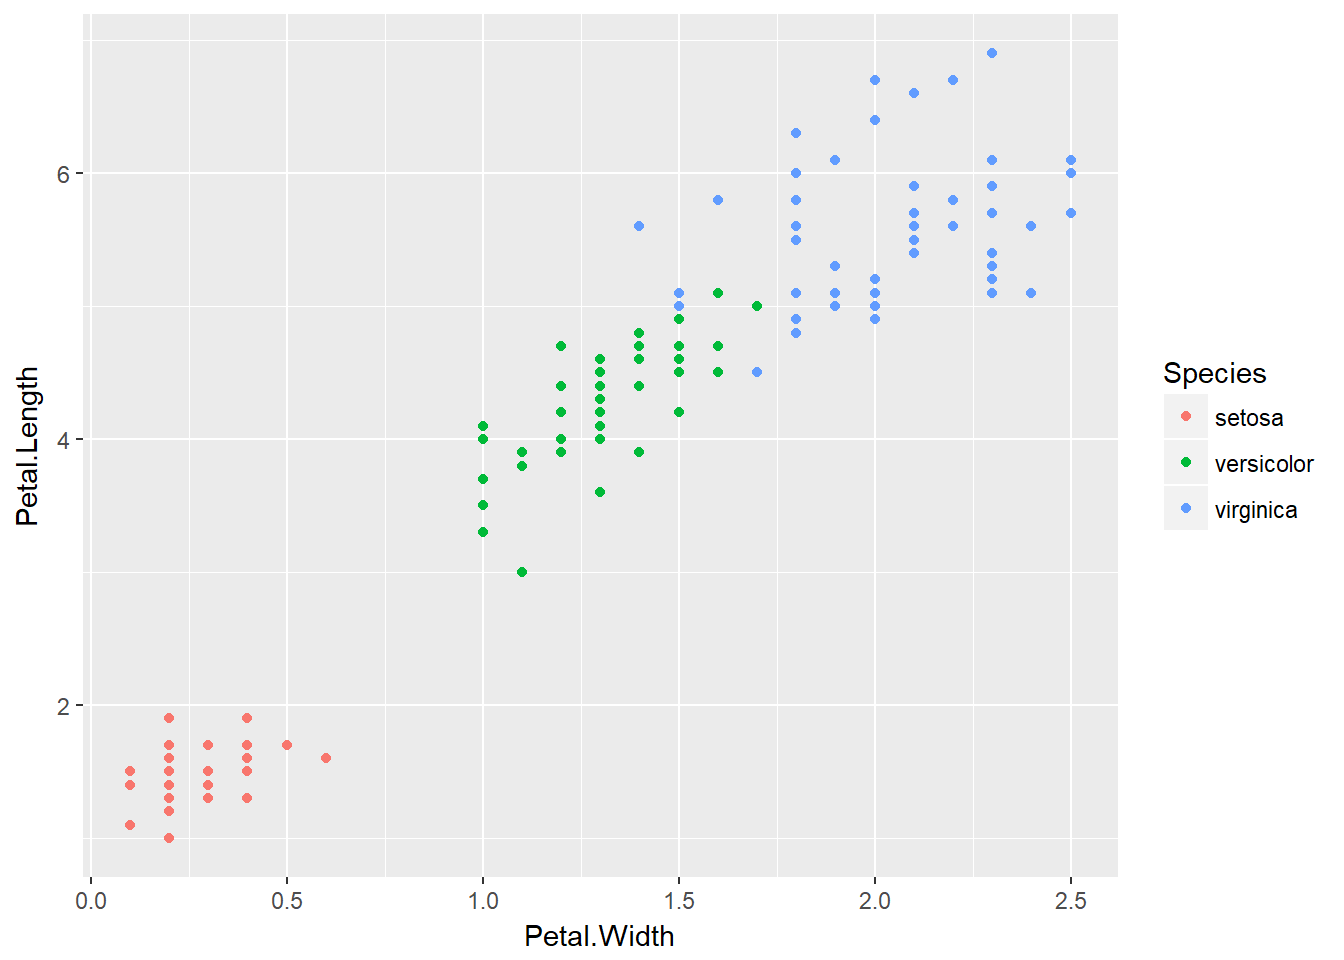
\includegraphics{02-Data_visu_files/figure-latex/desc1-1.pdf}

\begin{Shaded}
\begin{Highlighting}[]
\NormalTok{cars }\OperatorTok\StringTok{ }\KeywordTok{ggplot}\NormalTok{(}\KeywordTok{aes}\NormalTok{(}\DataTypeTok{x =}\NormalTok{ speed, }\DataTypeTok{y =}\NormalTok{ ..count..)) }\OperatorTok{+}\StringTok{ }\KeywordTok{geom_histogram}\NormalTok{(}\DataTypeTok{bins =} \DecValTok{10}\NormalTok{) }\OperatorTok{+}\StringTok{ }\KeywordTok{geom_density}\NormalTok{()}
\end{Highlighting}
\end{Shaded}

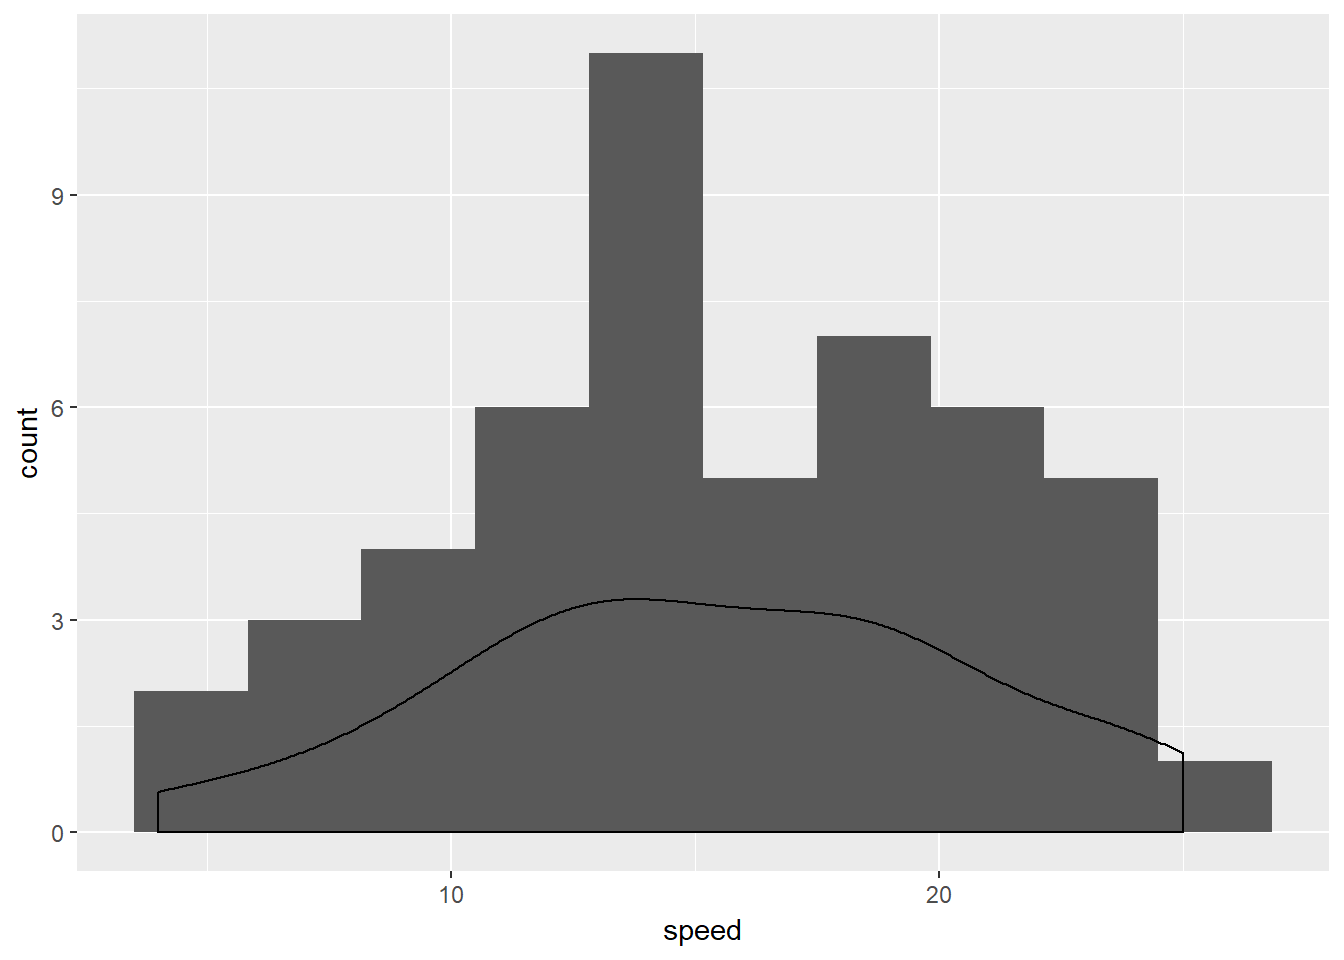
\includegraphics{02-Data_visu_files/figure-latex/desc1-2.pdf}

\begin{Shaded}
\begin{Highlighting}[]
\NormalTok{cars }\OperatorTok\StringTok{ }\KeywordTok{ggplot}\NormalTok{(}\KeywordTok{aes}\NormalTok{(}\DataTypeTok{x =}\NormalTok{ speed, }\DataTypeTok{y =}\NormalTok{ dist)) }\OperatorTok{+}\StringTok{ }\KeywordTok{geom_point}\NormalTok{() }\OperatorTok{+}\StringTok{ }\KeywordTok{geom_smooth}\NormalTok{(}\DataTypeTok{method =} \StringTok{"lm"}\NormalTok{)}
\end{Highlighting}
\end{Shaded}

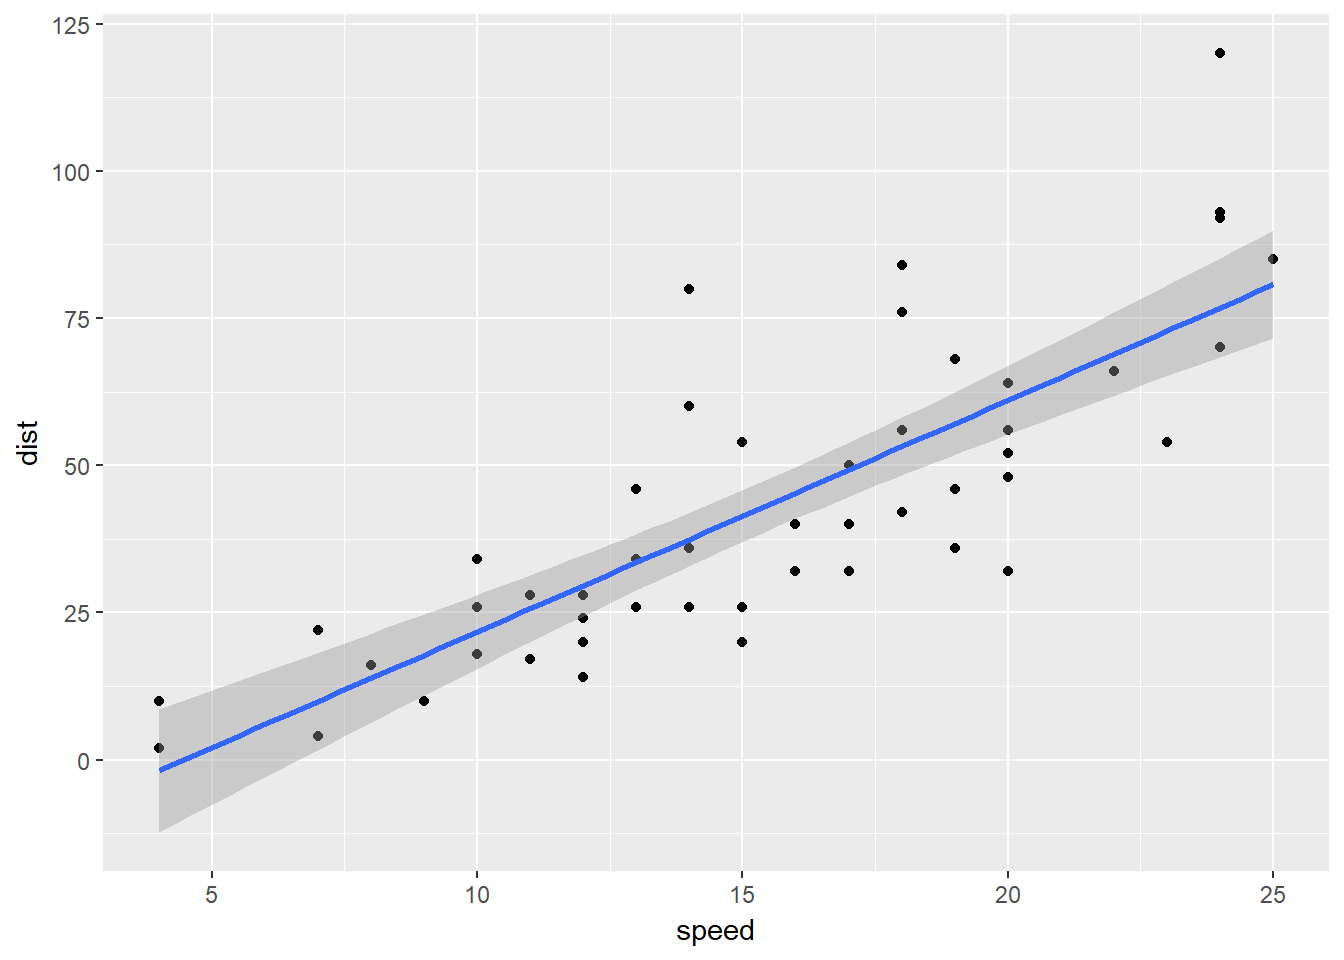
\includegraphics{02-Data_visu_files/figure-latex/desc1-3.pdf}

\begin{Shaded}
\begin{Highlighting}[]
\CommentTok{# If non linear smooth :  method = 'loess'}
\end{Highlighting}
\end{Shaded}

\begin{itemize}
\tightlist
\item
  \textbf{Multiple line}
\end{itemize}

\begin{Shaded}
\begin{Highlighting}[]
\NormalTok{longley }\OperatorTok\StringTok{ }\KeywordTok{ggplot}\NormalTok{(}\KeywordTok{aes}\NormalTok{(}\DataTypeTok{x =}\NormalTok{ Year)) }\OperatorTok{+}
\KeywordTok{geom_point}\NormalTok{(}\KeywordTok{aes}\NormalTok{(}\DataTypeTok{y =}\NormalTok{ Unemployed)) }\OperatorTok{+}
\KeywordTok{geom_point}\NormalTok{(}\KeywordTok{aes}\NormalTok{(}\DataTypeTok{y =}\NormalTok{ Armed.Forces), }\DataTypeTok{color =} \StringTok{"blue"}\NormalTok{) }\OperatorTok{+}
\KeywordTok{geom_line}\NormalTok{(}\KeywordTok{aes}\NormalTok{(}\DataTypeTok{y =}\NormalTok{ Unemployed)) }\OperatorTok{+}
\KeywordTok{geom_line}\NormalTok{(}\KeywordTok{aes}\NormalTok{(}\DataTypeTok{y =}\NormalTok{ Armed.Forces), }\DataTypeTok{color =} \StringTok{"blue"}\NormalTok{)}
\end{Highlighting}
\end{Shaded}

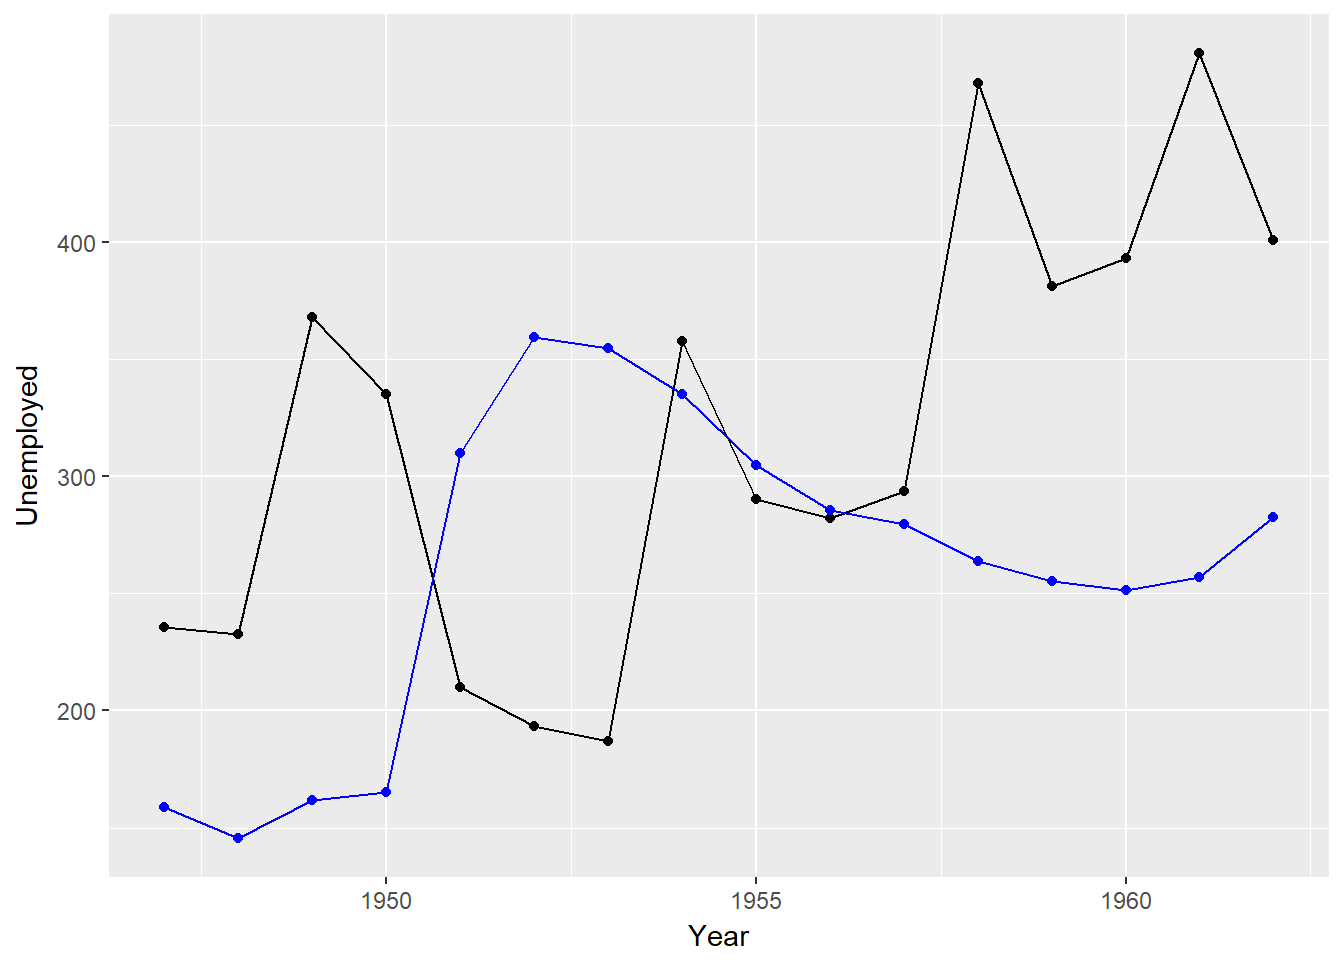
\includegraphics{02-Data_visu_files/figure-latex/desc2-1.pdf}

\begin{itemize}
\tightlist
\item
  \textbf{Scaling}
\end{itemize}

\begin{Shaded}
\begin{Highlighting}[]
\NormalTok{cars }\OperatorTok\StringTok{ }\KeywordTok{ggplot}\NormalTok{(}\KeywordTok{aes}\NormalTok{(}\DataTypeTok{x =}\NormalTok{ speed, }\DataTypeTok{y =}\NormalTok{ dist)) }\OperatorTok{+}
\KeywordTok{geom_point}\NormalTok{() }\OperatorTok{+}\StringTok{ }\KeywordTok{geom_smooth}\NormalTok{(}\DataTypeTok{method =} \StringTok{"lm"}\NormalTok{) }\OperatorTok{+}
\KeywordTok{scale_x_reverse}\NormalTok{(}\StringTok{"Speed"}\NormalTok{) }\OperatorTok{+}
\KeywordTok{scale_y_continuous}\NormalTok{(}\StringTok{"Stopping Distance"}\NormalTok{)}
\end{Highlighting}
\end{Shaded}

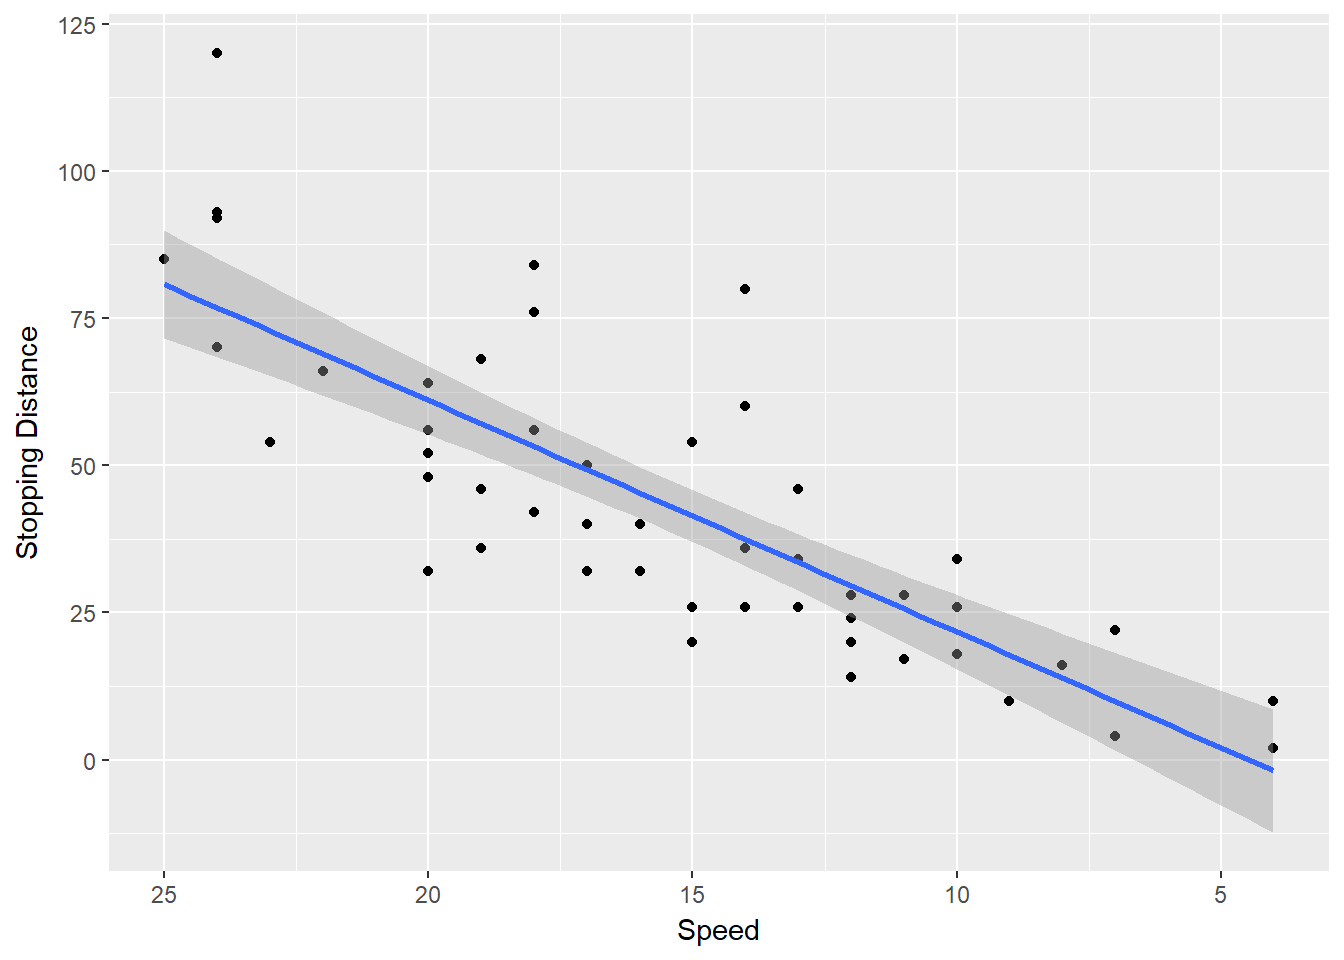
\includegraphics{02-Data_visu_files/figure-latex/scaling-1.pdf}

\begin{Shaded}
\begin{Highlighting}[]
\NormalTok{iris }\OperatorTok\StringTok{ }\KeywordTok{ggplot}\NormalTok{(}\KeywordTok{aes}\NormalTok{(}\DataTypeTok{x =}\NormalTok{ Species, }\DataTypeTok{y =}\NormalTok{ Petal.Length)) }\OperatorTok{+}
\KeywordTok{geom_boxplot}\NormalTok{() }\OperatorTok{+}\StringTok{ }\KeywordTok{geom_jitter}\NormalTok{(}\DataTypeTok{width =} \FloatTok{0.1}\NormalTok{, }\DataTypeTok{height =} \FloatTok{0.1}\NormalTok{) }\OperatorTok{+}
\KeywordTok{scale_x_discrete}\NormalTok{(}\DataTypeTok{labels =} \KeywordTok{c}\NormalTok{(}\StringTok{"setosa"}\NormalTok{ =}\StringTok{ "Setosa"}\NormalTok{,}
\StringTok{"versicolor"}\NormalTok{ =}\StringTok{ "Versicolor"}\NormalTok{,}
\StringTok{"virginica"}\NormalTok{ =}\StringTok{ "Virginica"}\NormalTok{))}
\end{Highlighting}
\end{Shaded}

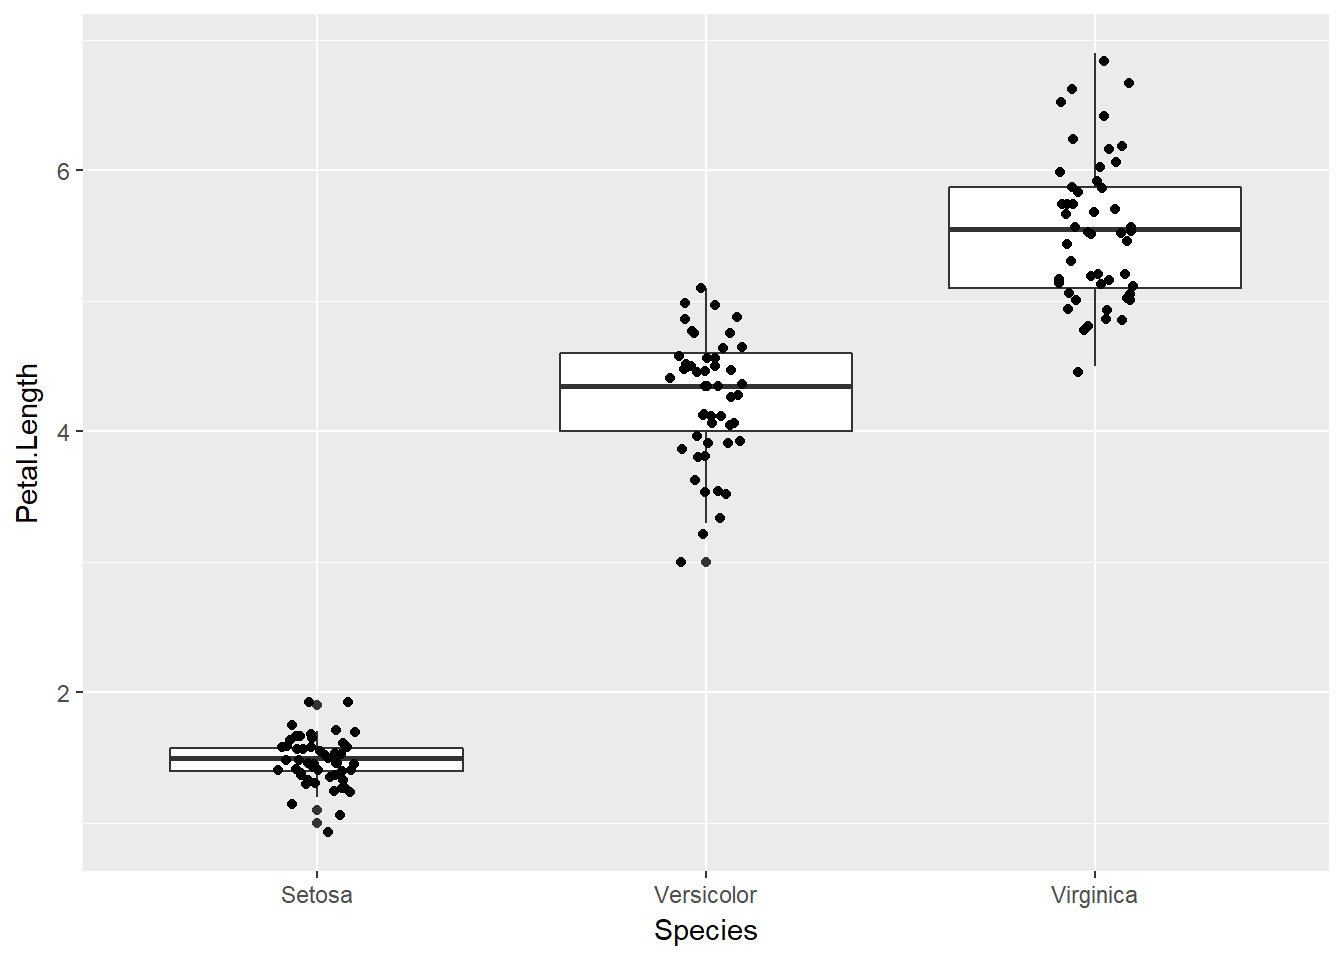
\includegraphics{02-Data_visu_files/figure-latex/scaling-2.pdf}

\begin{itemize}
\tightlist
\item
  \textbf{Correlation plot}

  \begin{itemize}
  \tightlist
  \item
    Pearson correlation : relation lin?aire
    \$\rho(X,Y)=\frac{E[(X-\mu_X)(Y-\mu_Y)]}{\sigma_X \sigma_Y} \$
  \end{itemize}
\end{itemize}

\begin{Shaded}
\begin{Highlighting}[]
\KeywordTok{library}\NormalTok{(corrplot)}
\NormalTok{correlation_world <-}\KeywordTok{read.csv}\NormalTok{(}\StringTok{"C:/Users/007/Desktop/Data science with R/R/Dataset/Chapter 4/Correlation/Correlation Data.csv"}\NormalTok{)}
\KeywordTok{corrplot}\NormalTok{(}\KeywordTok{cor}\NormalTok{(correlation_world[,}\DecValTok{2}\OperatorTok{:}\DecValTok{6}\NormalTok{],}\DataTypeTok{method =}\StringTok{"pearson"}\NormalTok{),}\DataTypeTok{diag =}\OtherTok{FALSE}\NormalTok{,}
\DataTypeTok{title =}\StringTok{"Correlation Plot"}\NormalTok{, }\DataTypeTok{method =}\StringTok{"ellipse"}\NormalTok{,}
\DataTypeTok{tl.cex =}\FloatTok{0.7}\NormalTok{, }\DataTypeTok{tl.col =}\StringTok{"black"}\NormalTok{, }\DataTypeTok{cl.ratio =}\FloatTok{0.2}
\NormalTok{)}
\end{Highlighting}
\end{Shaded}

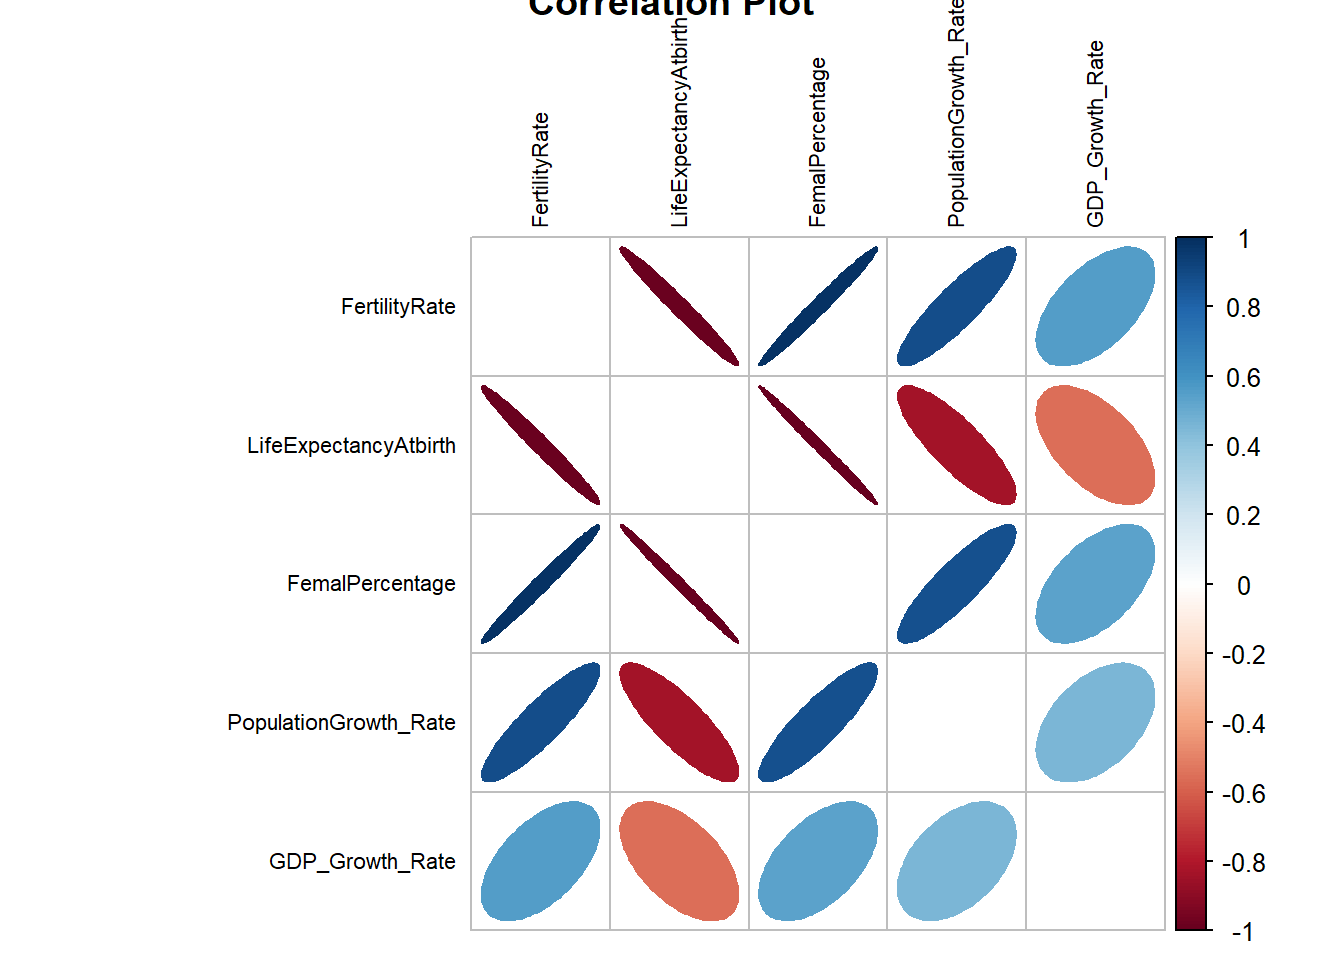
\includegraphics{02-Data_visu_files/figure-latex/corrplot-1.pdf}

\section{Spacial map}\label{spacial-map}

\begin{itemize}
\tightlist
\item
  \textbf{Static map}

  \begin{itemize}
  \tightlist
  \item
    qmap from ggplot
  \item
    Esay way : Machine learning with R, chap4
  \end{itemize}
\item
  \textbf{Interactive map : leaflet}

  \begin{itemize}
  \tightlist
  \item
    More information on \url{https://rstudio.github.io/leaflet}
  \item
    for more complex cartographie, check geoJSON
    \url{https://rstudio.github.io/leaflet/json.html}
  \item
    gps geolocalisation :
    \url{https://github.com/AugustT/shiny_geolocation}
  \end{itemize}
\end{itemize}

\begin{Shaded}
\begin{Highlighting}[]
\KeywordTok{library}\NormalTok{(leaflet)}

\NormalTok{lat =}\StringTok{ }\KeywordTok{seq}\NormalTok{(}\DecValTok{50}\NormalTok{, }\DecValTok{51}\NormalTok{ ,}\DataTypeTok{by=} \FloatTok{0.005}\NormalTok{)}
\NormalTok{lon =}\StringTok{ }\KeywordTok{seq}\NormalTok{(}\DecValTok{4}\NormalTok{,}\DecValTok{5}\NormalTok{, }\DataTypeTok{by=}\FloatTok{0.005}\NormalTok{)  }

\NormalTok{coords <-}\StringTok{ }\KeywordTok{as.data.frame}\NormalTok{(}\KeywordTok{cbind}\NormalTok{(}\DataTypeTok{Longitude =} \KeywordTok{sample}\NormalTok{(lon,}\DecValTok{50}\NormalTok{), }\DataTypeTok{Latitude =} \KeywordTok{sample}\NormalTok{(lat,}\DecValTok{50}\NormalTok{)))}
\NormalTok{coords}\OperatorTok{$}\NormalTok{V3  =}\StringTok{ }\KeywordTok{as.factor}\NormalTok{(}\KeywordTok{rep}\NormalTok{(}\StringTok{"Amandine"}\NormalTok{,}\DecValTok{50}\NormalTok{))}
\NormalTok{coords}\OperatorTok{$}\NormalTok{V4 =}\StringTok{ }\KeywordTok{rep}\NormalTok{(}\KeywordTok{seq}\NormalTok{(}\DecValTok{1}\NormalTok{,}\DecValTok{5}\NormalTok{,}\DataTypeTok{by=}\DecValTok{1}\NormalTok{),}\DecValTok{10}\NormalTok{)}

\CommentTok{# simple use}
\CommentTok{# Possibilité d'utilise d'autre map que google open street map}

\NormalTok{m <-}\StringTok{ }\KeywordTok{leaflet}\NormalTok{() }\OperatorTok\StringTok{ }\KeywordTok{setView}\NormalTok{(}\DataTypeTok{lng =} \FloatTok{4.8}\NormalTok{, }\DataTypeTok{lat =} \FloatTok{50.5}\NormalTok{, }\DataTypeTok{zoom =} \DecValTok{10}\NormalTok{)}
\NormalTok{m }\OperatorTok\StringTok{ }\KeywordTok{addProviderTiles}\NormalTok{(providers}\OperatorTok{$}\NormalTok{Stamen.Toner)}
\end{Highlighting}
\end{Shaded}

\includegraphics{02-Data_visu_files/figure-latex/leaflet-1.pdf}

\begin{Shaded}
\begin{Highlighting}[]
\NormalTok{m }\OperatorTok\StringTok{ }\KeywordTok{addProviderTiles}\NormalTok{(providers}\OperatorTok{$}\NormalTok{Esri.NatGeoWorldMap)}
\end{Highlighting}
\end{Shaded}

\includegraphics{02-Data_visu_files/figure-latex/leaflet-2.pdf}

\begin{Shaded}
\begin{Highlighting}[]
\CommentTok{# cartographe }
\KeywordTok{library}\NormalTok{(maps)}
\NormalTok{mapStates =}\StringTok{ }\KeywordTok{map}\NormalTok{(}\StringTok{"state"}\NormalTok{, }\DataTypeTok{fill =} \OtherTok{TRUE}\NormalTok{, }\DataTypeTok{plot =} \OtherTok{FALSE}\NormalTok{)}
\KeywordTok{leaflet}\NormalTok{(}\DataTypeTok{data =}\NormalTok{ mapStates) }\OperatorTok\StringTok{ }
\StringTok{      }\KeywordTok{addTiles}\NormalTok{() }\OperatorTok
\StringTok{      }\KeywordTok{addPolygons}\NormalTok{(}\DataTypeTok{fillColor =} \KeywordTok{topo.colors}\NormalTok{(}\DecValTok{10}\NormalTok{, }\DataTypeTok{alpha =} \OtherTok{NULL}\NormalTok{), }\DataTypeTok{stroke =} \OtherTok{FALSE}\NormalTok{)}
\end{Highlighting}
\end{Shaded}

\includegraphics{02-Data_visu_files/figure-latex/leaflet-3.pdf}

\begin{Shaded}
\begin{Highlighting}[]
\CommentTok{# modifier les markeret pop up }

\KeywordTok{leaflet}\NormalTok{(coords) }\OperatorTok\StringTok{ }\KeywordTok{addTiles}\NormalTok{() }\OperatorTok\StringTok{ }
\StringTok{  }\KeywordTok{addMarkers}\NormalTok{(}\DataTypeTok{clusterOptions =} \KeywordTok{markerClusterOptions}\NormalTok{(), }\DataTypeTok{popup =}\NormalTok{ coords}\OperatorTok{$}\NormalTok{V4)}
\end{Highlighting}
\end{Shaded}

\includegraphics{02-Data_visu_files/figure-latex/leaflet-4.pdf}

\begin{Shaded}
\begin{Highlighting}[]
\KeywordTok{leaflet}\NormalTok{(coords) }\OperatorTok\StringTok{ }\KeywordTok{addTiles}\NormalTok{() }\OperatorTok
\StringTok{  }\KeywordTok{addCircles}\NormalTok{(}\DataTypeTok{lng =} \OperatorTok{~}\NormalTok{Longitude, }\DataTypeTok{lat =} \OperatorTok{~}\NormalTok{Latitude, }\DataTypeTok{weight =} \DecValTok{1}\NormalTok{,}
             \DataTypeTok{radius =} \OperatorTok{~}\NormalTok{V4}\OperatorTok{^}\DecValTok{2} \OperatorTok{*}\StringTok{ }\DecValTok{30}\NormalTok{, }\DataTypeTok{popup =} \OperatorTok{~}\NormalTok{V3  )}
\end{Highlighting}
\end{Shaded}

\includegraphics{02-Data_visu_files/figure-latex/leaflet-5.pdf}

\begin{Shaded}
\begin{Highlighting}[]
\CommentTok{# rectangle zone}
\KeywordTok{leaflet}\NormalTok{() }\OperatorTok\StringTok{ }\KeywordTok{addTiles}\NormalTok{() }\OperatorTok
\StringTok{  }\KeywordTok{addRectangles}\NormalTok{(}
    \DataTypeTok{lng1=}\OperatorTok{-}\FloatTok{118.456554}\NormalTok{, }\DataTypeTok{lat1=}\FloatTok{34.078039}\NormalTok{,}
    \DataTypeTok{lng2=}\OperatorTok{-}\FloatTok{118.436383}\NormalTok{, }\DataTypeTok{lat2=}\FloatTok{34.062717}\NormalTok{,}
    \DataTypeTok{fillColor =} \StringTok{"transparent"}
\NormalTok{  )}
\end{Highlighting}
\end{Shaded}

\includegraphics{02-Data_visu_files/figure-latex/leaflet-6.pdf}


\end{document}
